\NeedsTeXFormat{LaTeX2e}[1995/12/01]
\documentclass[10pt]{bmc_article}    

\usepackage{cite} % Make references as [1-4], not [1,2,3,4]
\usepackage{url}  % Formatting web addresses  
\usepackage{ifthen}  % Conditional 
\usepackage{multicol}   %Columns
\usepackage[utf8]{inputenc} %unicode support
%\usepackage[latin1]{inputenc} %UNIX support if unicode package fails
\urlstyle{rm}
\usepackage[pdftex]{graphicx}
 
%\def\includegraphic{}
%\def\includegraphics{}

\setlength{\topmargin}{0.0cm}
\setlength{\textheight}{21.5cm}
\setlength{\oddsidemargin}{0cm} 
\setlength{\textwidth}{16.5cm}
\setlength{\columnsep}{0.6cm}

\newboolean{publ}

\newenvironment{bmcformat}{\begin{raggedright}\baselineskip20pt\sloppy\setboolean{publ}{false}}{\end{raggedright}\baselineskip20pt\sloppy}

%Publication style settings
%\newenvironment{bmcformat}{\fussy\setboolean{publ}{true}}{\fussy}

% Begin ...
\begin{document}
\begin{bmcformat}

\title{RDF in Chemistry}
 
\author{Egon L Willighagen\correspondingauthor$^{1}$%
       \email{Egon L Willighagen\correspondingauthor - egon.willighagen@ki.se}%
       and 
         Martin P Br\"andle$^2$%
         \email{Martin P Br\"andle - braendle@chem.ethz.ch}%
      }

\address{%
    \iid(1)Division of Molecular Toxicology, Institute of Environmental Medicine, Karolinska Institutet, SE-17177 Stockholm, Sweden\\
    \iid(2)Chemistry Biology Pharmacy Information Center, ETH Z\"urich, Z\"urich, Switzerland
}%

\maketitle


%\begin{abstract}
%        \paragraph*{Background:} Text for this section of the abstract. 
%        \paragraph*{Results:} Text for this section of the abstract \ldots
%        \paragraph*{Conclusions:} Text for this section of the abstract \ldots
%\end{abstract}

The American Chemical Society (ACS) Division of Chemical Information (CINF)
invited scientists from around the world to present their use of Resource
Description Framework (RDF) technologies in chemistry on 22nd-23rd August 2010
at the 240th ACS National Meeting in Boston, USA. During three half-day
sessions, the speakers demonstrated a mix of smaller and larger initiatives
where RDF and related technologies are used in cheminformatics and
bioinformatics as Open Standards for data exchange, common languages
(ontologies), and problem solving. (mb: tried to improve this phrase, since it
said before essentially the same thing as the previous sentence. Took text from
a later part). The fifteen presentations were grouped in the themes computation,
ontologies, and chemical applications. Figures 1 to 3 display the most important
keywords reflecting the abstracts of the talks in each session as word
clouds~\cite{WORDLE}.

The goal of the meeting was to make more chemists aware of what the RDF Open
Standard has to offer to chemistry. We are delighted to continue this effort
with this thematic issue, for which the speakers (and others) have been invited
to present their work in more detail to a wider chemistry community. The choice
of an Open Access journal follows this goal. The article processing charges for
this Thematic Series have been partially funded by Pfizer, Inc.  Pfizer, Inc.
has had no input into the content of the publication or the articles themselves.
 All articles in the series have been independently prepared by the authors and
have been subject to the journal's standard peer review process.

(mb: delete this part, moved to first paragraph) The meeting presented a mix of
smaller and larger initiatives and research projects where RDF technologies are
used as Open Standards for various tasks: data exchange, common languages
(ontologies), and problem solving. These tasks use various standards all based
on the underlying Resource Description Framework. (mb: /end delete)  In the
remainder of this editorial, we will briefly outline the various RDF
technologies and their use in chemistry, and introduce authors and their
contributions  

\section{Concepts}

The core RDF specification was introduced by the World Wide Web Consortium (W3C)
in 1999~\cite{Lassila1999} and defines the foundation for the RDF technologies. It has
evolved into a set of six recommendations by W3C published in 2004
(See Table~1). 
RDF specifies a very simple data structure linking an subject to an object or a
value (literal) using a predicate. Cheminformaticians will recognize this data
structure as an edge from graph theory. This structure allows us to represent
facts like “vanillin dissolves in methanol”~\cite{ONS2010}. Now, RDF uses Uniform
Resource Identifiers (URIs) to identify things. Therefore, the RDF equivalent of
the solution statement could be like this so-called triple:

http://dbpedia.org/resource/Vanillin http://example.com/dissolvesIn http://dbpedia.org/resource/Methanol

Those who know a bit about how web pages link to each other, may also recognize
this data structure as a hyperlink. This is not surprising, since RDF is the
core technology behind the proposed Semantic Web~\cite{BER2001}. In fact, web
nature is clear here, as one can use the URIs for vanillin and methanol to
get further information on those two chemicals, by following the link
by which they are represented. These molecules' URIs are said to be
dereferencable, allowing to spider the web for information following
the hyperlinks, quite like how you follow hyperlinks on web sites.
Hence, the term Semantic Web.

Recent projects such as Bio2RDF~\cite{BEL2008}, Chem2Bio2RDF~\cite{CHE2010},
and OpenTox~\cite{Hardy2010} have brought genomic, pharmaceutical and
chemical knowledge to the Semantic Web by expressing it in RDF.
These three projects aim at making databases with chemical knowledge
available from a central access point, interlinking the individual
data sets. Smaller data sets are also becoming available as RDF, such as
the Open Notebook Science Solubility data~\cite{citeulike:5441072}.

(mb: will continue here Monday evening)

FIXME - more work to be done to bring chemical compound databases and chemical names
to RDF; I see a gap there. In as far are PubChem and other repositories RDFised?

\section{Formats}

The actual use of RDF depends on various further standards. For example, we need
standards that describe the syntax by which RDF statements are exchanged, and
various have been defined: RDF/XML is a XML-based serialization [], while
simpler formats exist with N-Triples [] and Notation3 []. For integration with
current web practises RDFa has been defined to allow RDF triples to be embedded
in HTML pages~\cite{RDFA2008}. Additionally, several proposals have been written that
describe how RDF can be serialized JavaScript Object Notation (JSON) []. Several
of these standards are used in the papers in this Series.

Using these serializations, RDF can be downloaded directly from pure RDF
documents (RDF/XML, Notation3), or extracted from RDFa-based webpages using
online RDF extraction web services, like http://www.w3.org/2007/08/pyRdfa/.
These approaches make it simple to aggregate chemical data from the web.
However, we also increasingly see RDF provided as a queriable database. …
SPARQL....

[ADD SCREENSHOT OF RDFa EXAMPLE]

\section{Ontologies}

With RDF we have a data structure to link resources and provide details about
those resources. The next standard we will discuss now is the Web Ontology
Language (OWL) which brought the RDF technology to the ontology community~\cite{GUN2004}.
Ontologies are most certainly not new to chemistry, or biology or life sciences,
but the OWL standard makes it much easier to use ontologies. Ontologies, like
controlled vocabularies and thesauri, describe what things mean, by linking
terms to a human-readable definition. As such, ontologies are used for sharing
knowledge in a common language, as well as to organize that knowledge []. 

[CITE WORK DUMONTIER AND OTHERS]

FIXME:
- OWL at present used to build up ontologies. These are used at present to
interlink facts from different domains. 
- problem of mapping different ontologies - should the cheminformatics community
work towards a standard. How are standards organizations in chemistry (IUPAC,
NIST etc.) taking up?
- we are at present not at the point where chemical inferencing is done using
RDF and OWL. Further work to be expected here


\section{Querying the World Wide Web}

The most promising technologies in the RDF family is the
SPARQL Query Language for RDF (SPARQL)~\cite{PrudHommeaux2008}, which has been
used by Chen et al. in three chemogenomics use cases~\cite{CHE2010}. 
One of the use cases shows ... "PubChem compounds (e.g. CID 5754) are identifiedthat are active in bioassays that are associated with protein targets, which are associated with genes (via UNIPROT), which are identified as those with which Dexamethasone interacts (via DrugBank). The resultant compounds are thus those that have a similar activity profile to Dexamethasone."

A second use case shows ... "The drugs that are associated with hepatotoxicity-related side effects are associated with their targets using DrugBank. The targets are associated with pathways using KEGG to establish association chains between pathways and side-effects."

Chen's Chem2Bio2RDF database aggregated RDF versions of various chemogenomics databases
into one queryable repository. However, SPARQL also allows setting up federated
queries that can retrieve information from different remote database at the same
time, as was recently shown by Cheung et al.~\cite{Cheung2009}

\section{Outlook}

(mb: Egon, I think here we should summarize the status and give some outlook, eg. 
- I see a need for statistical tools that can
extract/aggregate/cluster/visualize RDF data in a chemical context
- I see a problem with RDF to describe data that has multi-dimensional
relations. In essence, an RDF triple describes a single relation. This works
well for chemical descriptors that are one-dimensional, e.g. SubstanceX
hasMeltingPoint 128degreeCelsisus. However, in physical and quantum chemistry,
we have a lot of descriptors that are arrays or tensors, and you need a
double/triple/multi-relation to describe an element of the array or tensor. Of
course one can split down to several RDF triples (as one splits down a
n:m-relation in a relational database by using a connection table that is
inserted into the database scheme with 1:n and 1:m relations), but this gets
very cumbersome. This is why I and a research group at ETH (H.-P. Lüthi group)
hesitate to switch to RDF for describing quantum chemical data.)


\ifthenelse{\boolean{publ}}{\begin{multicols}{2}}{}


{\ifthenelse{\boolean{publ}}{\footnotesize}{\small}
 \bibliographystyle{bmc_article}  % Style BST file
  \bibliography{editorial} }     % Bibliography file (usually '*.bib' ) 

%%%%%%%%%%%

\ifthenelse{\boolean{publ}}{\end{multicols}}{}

\clearpage

\section*{Figures}
  \subsection*{Figure 1 - Keyword cloud for the \textit{RDF and Computation} session.}
  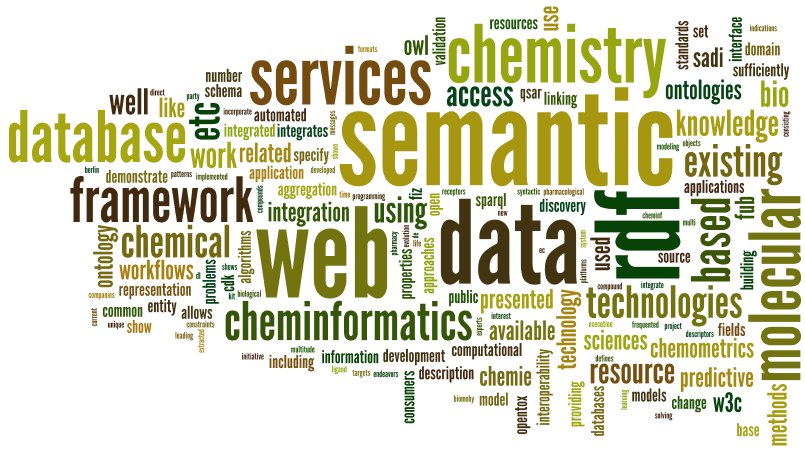
\includegraphics[width=0.5\textwidth]{graphics/wordle_cinf003} 

  \subsection*{Figure 2 - Keyword cloud for the \textit{RDF and Ontologies} session.}
  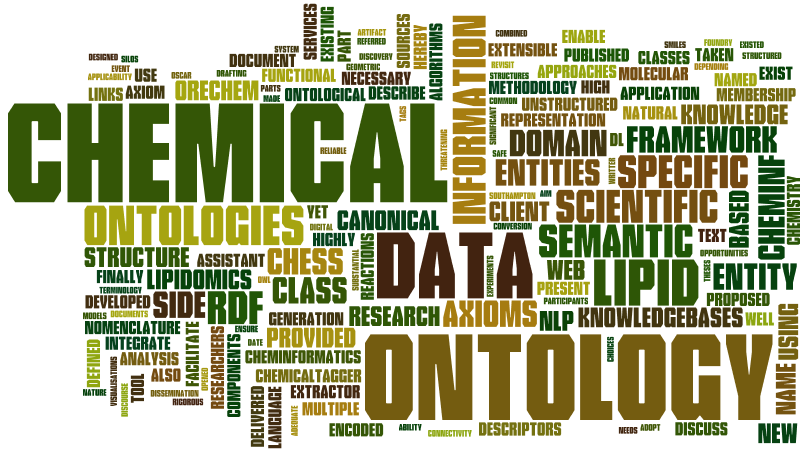
\includegraphics[width=0.5\textwidth]{graphics/wordle_cinf0031} 

  \subsection*{Figure 3 - Keyword cloud for the \textit{RDF and Chemical Applications} session.}
  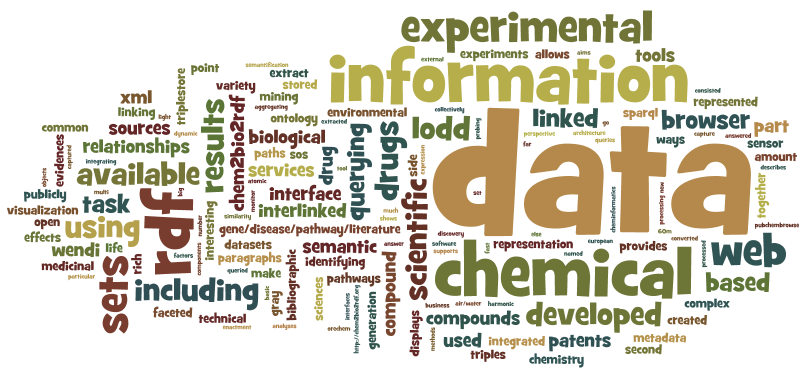
\includegraphics[width=0.5\textwidth]{graphics/wordle_cinf0032} 

\clearpage

\section*{Tables}
  \subsection*{Table 1 - Key W3C Specifications}
    Several of the key specifications and when they were
    recommended by the World Wide Web Consortium. \par \mbox{}
    \par
    \mbox{
      \begin{tabular}{lll}
        Year & Technology & Description \\ 
        \hline
        1999 & RDF     & Resource Description Framework (RDF) Model and Syntax Specification~\cite{Lassila1999} \\
        2004 & RDF/XML & RDF/XML Syntax Specification (Revised)~\cite{Beckett2004} \\
             & RDF     & Resource Description Framework (RDF): Concepts and Abstract Syntax~\cite{Carroll2004}  \\
             & OWL     & OWL Web Ontology Language Overview~\cite{OWL22009}\\
        2007 & OWL2    & OWL 2 Web Ontology Language Document Overview~\cite{OWL22009}  \\
        2008 & RDFa    & RDFa in XHTML: Syntax and Processing~\cite{RDFA2008} \\
             & SPARQL  & SPARQL Query Lanuage for RDF~\cite{PrudHommeaux2008} \\
      \end{tabular}
      }


\end{bmcformat}
\end{document}







